% vim: set tw=80 aw sw=2 sts=2 noet:
\documentclass{beamer}

%\includeonlyframes{c} % speeding up compilation speed during debug

\usepackage[utf8x]{inputenc} % diacritice
\PrerenderUnicode{ĂăâÂîÎșȘțȚ}
\usepackage[romanian]{babel}
\usepackage{hyperref}        % \url{http://...} | \href{http://...}{Nume Link}

% Pentru a include cod decomentati urmatoarele 3 linii
%\usepackage{color}			 % highlight
%\usepackage{alltt}			 % highlight
%\usepackage{code/highlight}	 % highlight

\mode<presentation>
\usetheme{SCS}

% Pentru a afisa (cont.) la slide-uri prea lungi split-uite pe mai multe pag
\setbeamertemplate{frametitle continuation}[from second]
% Pentru a modifica modul de afisare al numerelor de slide
\setbeamertemplate{footline}[frame number]

\title{Malspec: Malicious Application Analysis}
\subtitle{Bachelor Thesis, July 2013}
% Folositi institutul pentru conducatorul stiintific
\institute{As.dr.ing. Laura Gheorghe}
\author{Cristian Condurache}

\begin{document}

{
  % Schimbam fundalul aici pentru a avea slide-ul cu logo-urile
  % Nu știu momentan cum se face asta în template.
  \usebackgroundtemplate{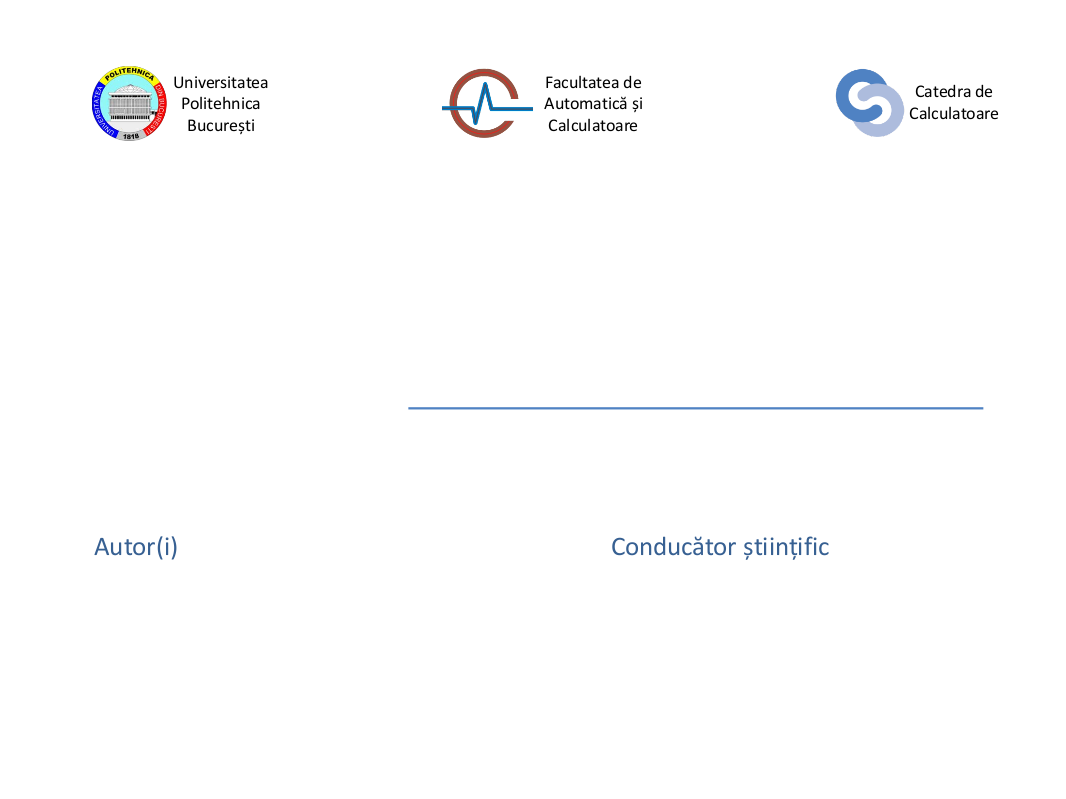
\includegraphics[width=\paperwidth]{title}}
  \frame{\titlepage}
}

\begin{frame}{Motivation \& Goals}
  \begin{itemize}
    \item Why?
    \begin{itemize}
      \item[--] Popularity of Linux based OS
      \item[--] Use in embedded systems
    \end{itemize}
    \item How?
    \begin{itemize}
      \item[--] Malicious behavior pattern mining
    \end{itemize}
  \end{itemize}
\end{frame}

\begin{frame}{Malware Detection}
  \begin{itemize}
    \item Signature-based
    \begin{itemize}
      \item[--] Problem: fails to detect new malware, obfuscation
    \end{itemize}
    \item Behavior-based
    \begin{itemize}
      \item[--] Problem: behavior patterns require manual identification
    \end{itemize}
  \end{itemize}
\end{frame}

\begin{frame}{Malspec Mining Algorithm}
  \begin{itemize}
    \item Input: a malware sample and a set of benign programs
    \item Output: a malicious behavior pattern
    \item Creates a graph for each program
    \begin{itemize}
      \item[--] A node represents a system call
      \item[--] An edge is an argument dependency
    \end{itemize}
    \item Computes malware specifications as ``difference'' between graphs
    \begin{itemize}
      \item[--] Maximal common subgraph algorithm
      \item[--] Complement graph
      \item[--] Minimal transversal
    \end{itemize}
  \end{itemize}
\end{frame}

\begin{frame}{Dependency Graph}
  \begin{itemize}
    \item Initial nodes
  \end{itemize}
  \begin{figure}[p]
    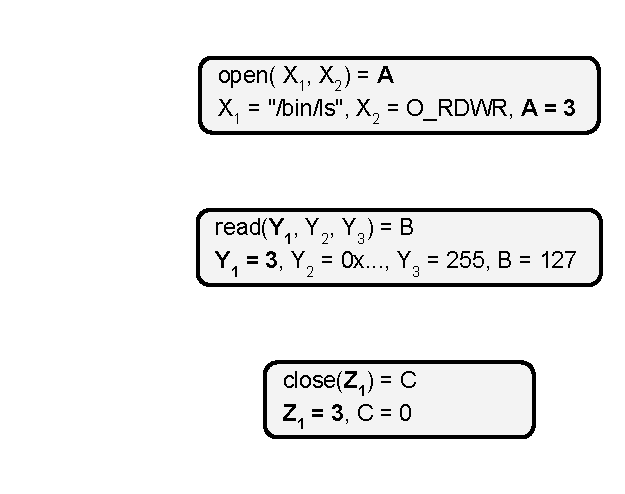
\includegraphics[width=3in]{img/syscall-dep-graph-0.pdf}
    \end{figure}
\end{frame}

\begin{frame}{Dependency Graph}
  \begin{itemize}
    \item Adding dependency edge between open and read
  \end{itemize}
  \begin{figure}[p]
    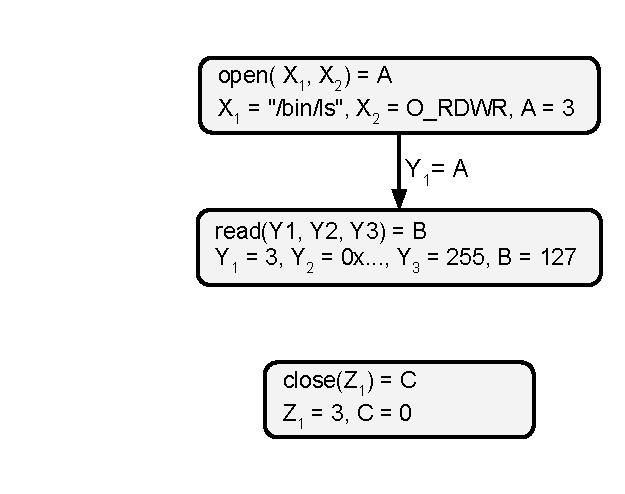
\includegraphics[width=3in]{img/syscall-dep-graph-1.pdf}
%    \caption{}
    \end{figure}
\end{frame}

\begin{frame}{Dependency Graph}
  \begin{itemize}
    \item Adding dependency edge between open and close
  \end{itemize}
  \begin{figure}[p]
    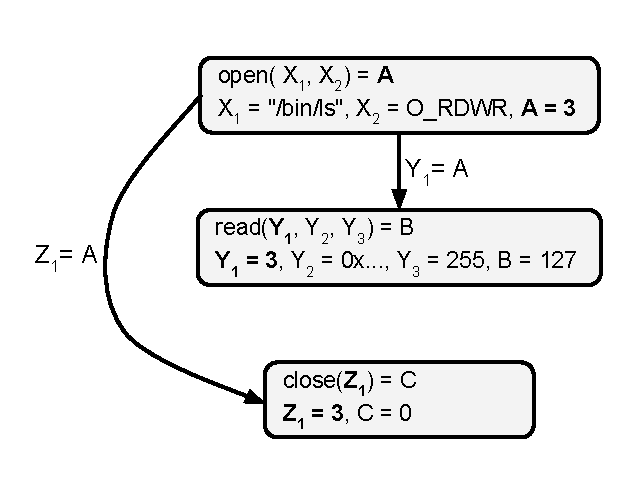
\includegraphics[width=3in]{img/syscall-dep-graph-2.pdf}
%    \caption{}
    \end{figure}
\end{frame}

\begin{frame}{Malsharp Architecture}
  \begin{figure}[p]
    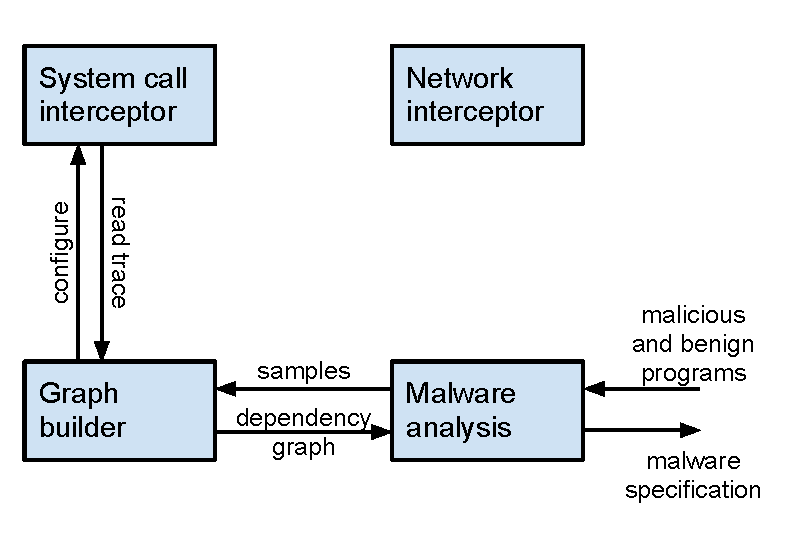
\includegraphics[width=4in]{img/mal-sharp-architecture.pdf}
    \end{figure}
\end{frame}

\begin{frame}{Implementation (1)}
  \begin{itemize}
    \item System Call Interceptor Driver (SCID)
    \begin{itemize}
      \item[--] Logs execution trace for a process
      \item[--] Kernel module, registers by using miscdevice
      \item[--] Controlled via the ioctl system call
    \end{itemize}
    \item Network Interceptor (NI)
    \begin{itemize}
      \item[--] Uses netfilter hooks to monitor traffic
      \item[--] Can be configured to monitor specific protocols
      \item[--] Statistics can be read from /proc/interceptor
    \end{itemize}
  \end{itemize}
\end{frame}

\begin{frame}{Implementation (2)}
  \begin{itemize}
    \item Graph Builder
    \begin{itemize}
      \item[--] Runs each program
      \item[--] Reads execution traces from SCID
      \item[--] Finds argument dependencies
    \end{itemize}
    \item Malware Analysis
    \begin{itemize}
      \item[--] Uses the graph builder for each program
      \item[--] Applies the malspec mining algorithm
    \end{itemize}
  \end{itemize}
\end{frame}

\begin{frame}{Evaluation (1)}
  \begin{itemize}
    \item Virtual machine, snapshots
    \item Revert to snapshot before each test
    \item Bridged network access
    \item A set of known malware samples
    \begin{itemize}
      \item[--] Viruses: Virus.Linux.Rike.1627, Virus.Linux.Osf.8759
      \item[--] Backdoor: Backdoor.Linux.CGI, Backdoor.Linux.Phobi.1
    \end{itemize}
  \end{itemize}
\end{frame}

\begin{frame}{Evaluation (2)}
  \begin{itemize}
    \item Execution traces and graphs successfully built
    \item Small malware patterns identified, 3-5 nodes
    \item Node aggregation reduced total number of nodes in large graphs by 25-30\%
  \end{itemize}
\end{frame}

\begin{frame}{Evaluation (3)}
  \begin{itemize}
    \item Node aggregation results
  \end{itemize}
  \begin{figure}[p]
    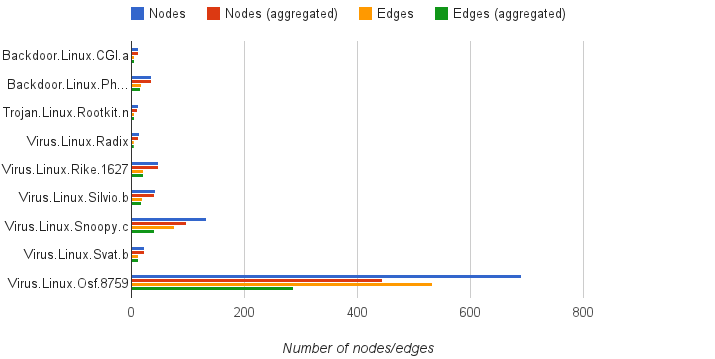
\includegraphics[width=4in]{img/node-aggregation-android.png}
  \end{figure}
\end{frame}

\begin{frame}{Conclusions}
  \begin{itemize}
    \item Proof of concept for a Linux malware behavior miner
    \item Node aggregation successfully reduced total number of nodes
    \item Possible future improvements:
    \begin{itemize}
      \item[--] Additional pruning: node ordering strategies
      \item[--] Adding other types of dependency edges
    \end{itemize}
  \end{itemize}
\end{frame}

% ------------------------------------------------
%                    BONUS
% ------------------------------------------------

\begin{frame}{Test programs}
  \begin{figure}[p]
    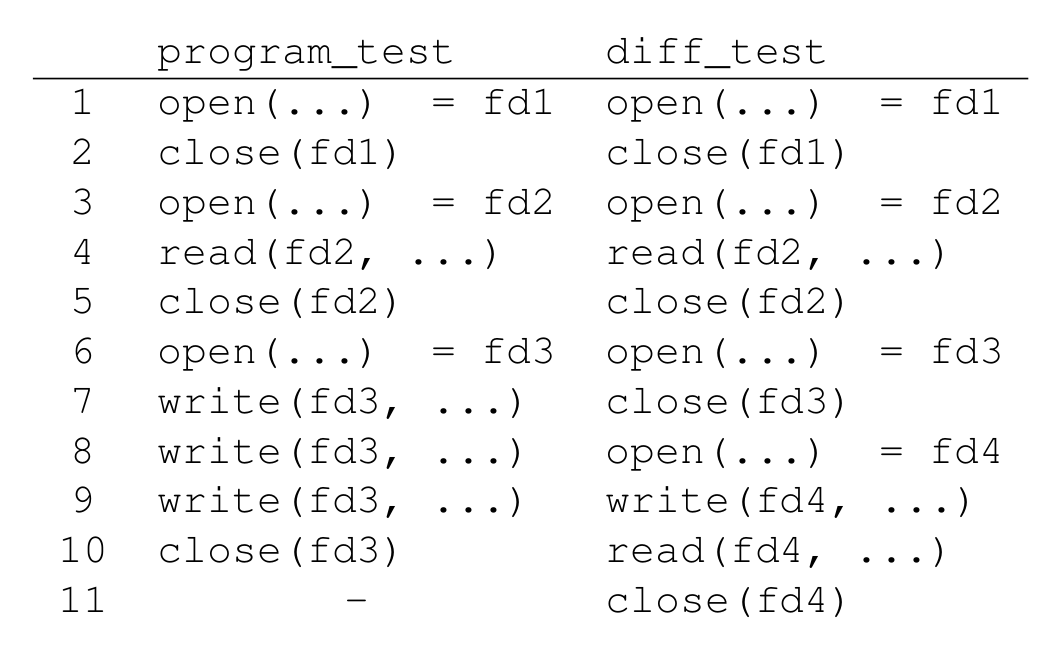
\includegraphics[width=3.6in]{img/programs.png}
%    \caption{}
    \end{figure}
\end{frame}

\begin{frame}{Maximal common edge set}
  \begin{figure}[p]
    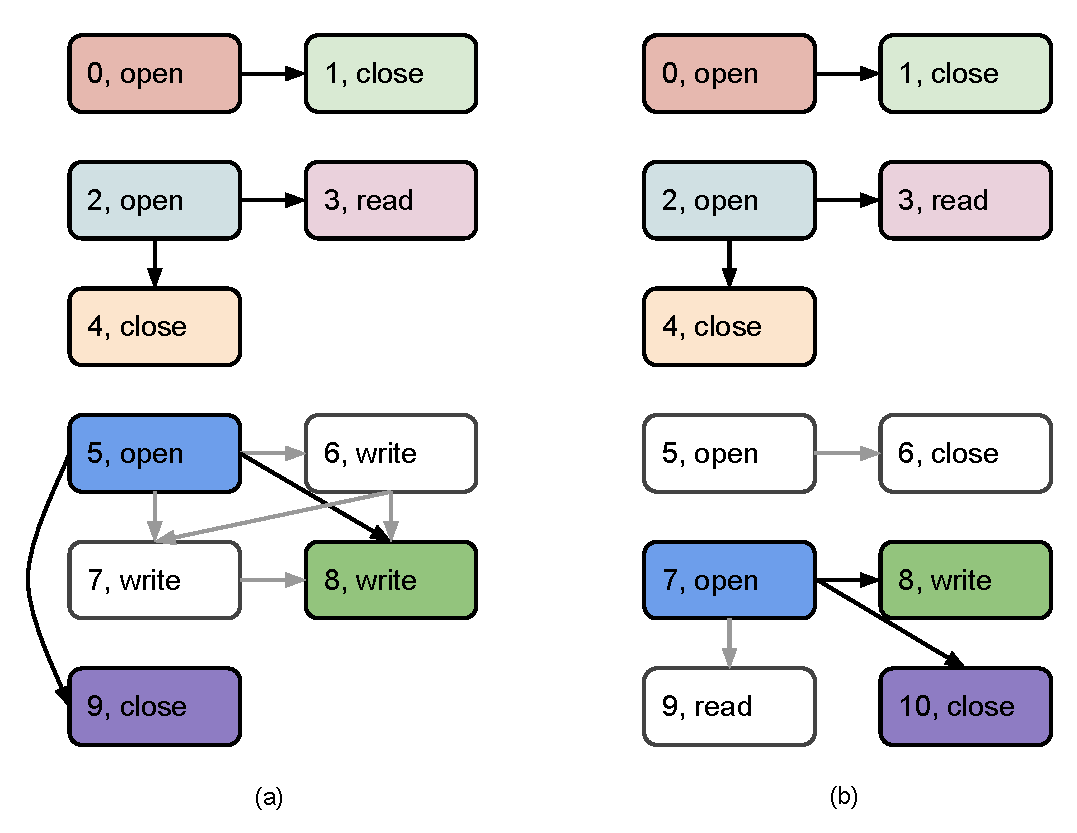
\includegraphics[width=3.6in]{img/max-common-edge-set.pdf}
%    \caption{}
    \end{figure}
\end{frame}

\begin{frame}{Complement and minimal transversal}
  \begin{figure}[p]
    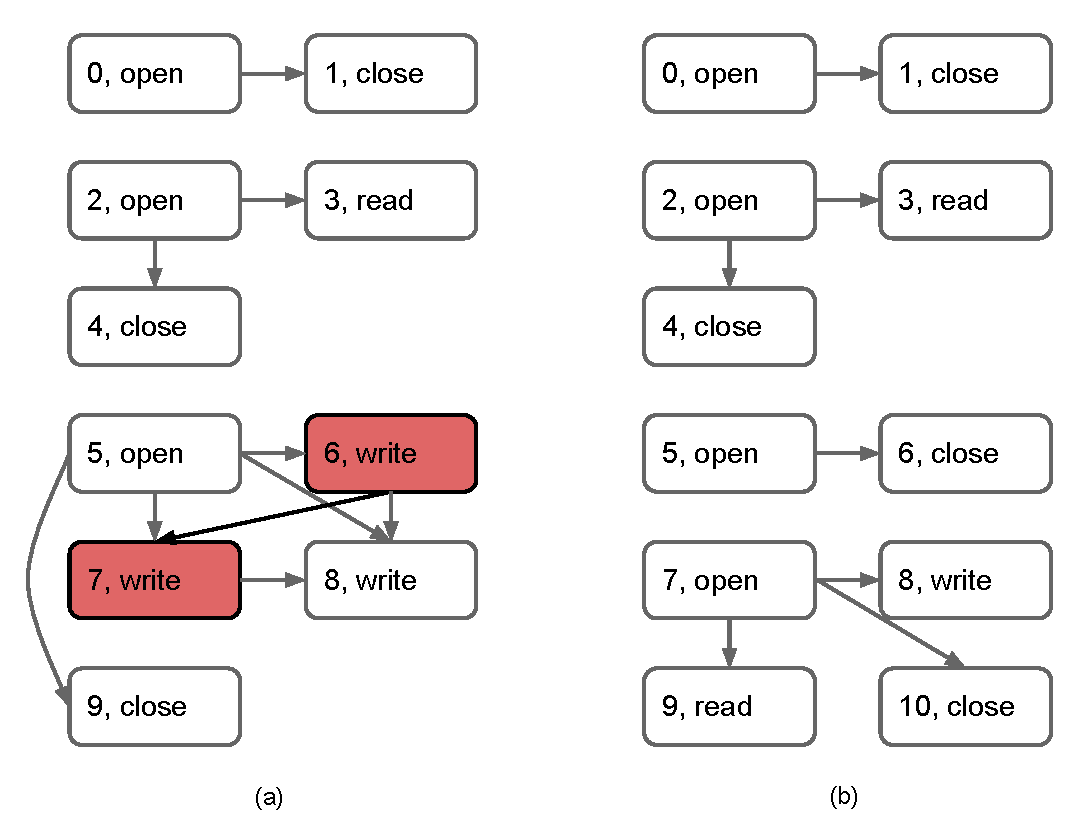
\includegraphics[width=3.6in]{img/min-transversal-compl.pdf}
%    \caption{}
    \end{figure}
\end{frame}

\end{document}

